\subsection{Specifying models using \texttt{lme4} in \texttt{R}}
\label{sec:specifyingmodelsusinglme4inr}

This section and the next focus on \texttt{lme4}, an often used package to do multilevel modeling in \texttt{R} with maximum likelihood methods \citep{BatesEa2015}.
The data set used to illustrate the process of fitting GLMMs in \texttt{R} is taken from \citet{Schaefer2018}.

\subsubsection{Overview of the data set}

The data used here for illustration purposes comes from \citet{Schaefer2018}, where a binary case alternation in German measure phrases is modelled.
In the first alternant, the kind-denoting noun (here \textit{Wein} `wine') is in the genitive as in (\ref{ex:intro:alternation1}).
In the second alternant, the kind-denoting noun is assigned the same case as the head measure noun as in (\ref{ex:intro:alternation2}).

\begin{exe}
  \ex\label{ex:intro:alternation}
  \begin{xlist}
    \ex[ ]{\label{ex:intro:alternation1} \gll Wir trinken [[ein Glas]\Sub{Acc} [guten Weins]\Sub{Gen}]\Sub{Acc}.\\
    we drink a glass good wine \\
    \glt We drink a glass of good wine.}
    \ex[ ]{\label{ex:intro:alternation2} Wir trinken [[ein Glas]\Sub{Acc} [guten Wein]\Sub{Acc}]\Sub{Acc}.}
  \end{xlist}
\end{exe}

The influencing first-level factors derived from theory-driven analysis and previous accounts comprise the numeric stylistic indicator variables \texttt{Badness} (a measure of document quality) and \texttt{Genitives} (a measure of the frequency of genitives), a binary variable \texttt{Cardinal} encoding whether the NP is modified by a cardinal or not, and the three-level variable \texttt{Measurecase} encoding the case of the head noun.
Furthermore, there are two crossed random intercepts for the kind noun (\texttt{Kindlemma}) and the measure noun (\texttt{Measurelemma}).
These random intercepts come with second-level models including a number of fixed second-level effects.
For \texttt{Kindlemma}, there are: \texttt{Kindfreq} (numeric, z-transformed), which encodes the lemma frequency; \texttt{Kindgender} (binary), which encodes the grammatical gender of the kind noun; \texttt{Kindattraction} (numeric, z-transformed), which encodes the influence of neighbouring constructions.
For \texttt{Measurelemma}, there are: \texttt{Measurefreq} and \texttt{Measureattraction}, which correspond to the similarly named variables for \texttt{Kindlemma}; \texttt{Measureclass} (5-level categorical), which encodes the broad semantic class of the measure noun.
Finally, the dependent variable \texttt{Construction} is coded as 1 if the genitive is used and as 0 if there is case identity.

\subsubsection{A simple varying intercept instead of a fixed effect}

\paragraph{Fitting and evaluating the model}

First, it is shown how a grouping factor can be specified as a fixed or a random effect.
The following is the standard \texttt{glm()} call to estimate a model with the measure lemma (150 levels) as a fixed effect.
For illustration purposes, not all available regressors are used here.

\vspace{0.5\baselineskip}

\begin{lstlisting}
glm.01 <- glm(Construction~1
              +Measurelemma
              +Badness
              +Cardinal
              +Genitives
              +Measurecase,
	      data=measure,
	      family=binomial(link=logit))
\end{lstlisting}

The output of the \texttt{summary(glm.01)} command (not shown here) shows that the estimates for the 149 fixed effects corresponding to \texttt{Measurelemma} have extremely high standard errors and are virtually unusable.
The Nagelkerke coefficient of determination for this model can be calculated using the \texttt{NagelkerkeR2(glm.01)} function from the \texttt{fmsb} package, and it is 0.397.

However, the grouping factor \texttt{Measurelemma} is not suitable for use as a fixed effect, and the following specification re-estimates the model as a GLMM using the \texttt{glmer} function with \texttt{Measurelemma} as a varying intercept.

\vspace{0.5\baselineskip}

\begin{lstlisting}
glmm.01 <- glmer(Construction~1
                 +(1|Measurelemma)
                 +Badness
                 +Cardinal
                 +Genitives
                 +Measurecase,
                 data=measure,
		 family=binomial(link=logit))
\end{lstlisting}

The output of the \texttt{summary(glmm.01)} command looks as follows (abbreviated).

\vspace{0.5\baselineskip}

\begin{lstlisting}
Random effects:
 Groups       Name        Variance Std.Dev.
 Measurelemma (Intercept) 1.252    1.119   
Number of obs: 5063, groups:  Measurelemma, 150

Fixed effects:
               Estimate Std. Error z value Pr(>|z|)    
(Intercept)    -2.32135    0.17867 -12.992  < 2e-16 ***
Badness        -0.14065    0.04474  -3.144  0.00167 ** 
CardinalNo      1.35673    0.13947   9.727  < 2e-16 ***
Genitives      -0.73886    0.04239 -17.429  < 2e-16 ***
MeasurecaseAcc -0.01923    0.08821  -0.218  0.82740    
MeasurecaseDat  0.25047    0.12045   2.079  0.03758 *  
\end{lstlisting}

\texttt{R} outputs the standard coefficient table for the fixed effects including the overall intercept.
Above this coefficient table, there is a summary of the random effects.
The number of groups for \texttt{Measurelemma} is correctly given as 150, and the variance in the random intercepts is 1.252.%
\footnote{The variance-covariance matrix of GLMMs can also be extracted directly using the \texttt{VarCorr(glmm.01)} command.}
As a rule of thumb, the larger is the variance between the intercepts, the larger are the differences between the groups.
For the variance estimate, confidence intervals can be obtained with either one of the following commands, where the first one uses the profile method (based on likelihood ratio tests) and the second one uses the parametric bootstrap, which is sometimes considered more robust.%
\footnote{Since the bootstrap (especially with smaller original sample sizes) tends to run into replications where the estimation of the variance fails and is thus returned as 0, the bootstrap interval is sometimes skewed towards 0 when the profile confidence interval frames the true value symmetrically. The bootstrap is thus not always more robust or intrinsically better.
Comparing both methods is recommended.}

\vspace{0.5\baselineskip}

\begin{lstlisting}
confint(glmm.01, parm="theta_", method="profile")
confint(glmm.01, parm="theta_", method="boot", nsim = 250)
\end{lstlisting}

For the first command, the output (95\% confidence interval) is 0.887 and 1.414.
Without applying formal significance testing, this is a reasonably narrow interval, and it does not extend to 0.
It is generally not a good idea to do (stepwise) model selection for random effects.
Even worse, while bootstrap methods are available for the comparison of two nested mixed models (see below), the comparison of a GLM and a GLMM (which extends the GLM by one random effect) is mostly uncharted territory and should be avoided.

Single conditional modes for the levels of the grouping factor can be extracted using the \texttt{ranef} command.
The following command stores a list of conditional modes for \texttt{Measurelemma} in \texttt{glmm.01.ranef}.

\vspace{0.5\baselineskip}

\begin{lstlisting}
glmm.01.ranef <- ranef(glmm.01, condVar = TRUE,
                       drop = TRUE)$Measurelemma
\end{lstlisting}

If the options \texttt{condVar = TRUE} and \texttt{drop = TRUE} are passed as above, then conditional variance-covariance estimates are returned as attributes of the result.
They have to be accessed using the \texttt{attributes} function as shown below.

\vspace{0.5\baselineskip}

\begin{lstlisting}
attributes(glmm.01.ranef)$postVar
\end{lstlisting}

These can be used to construct prediction intervals around the predicted conditional modes in order to display them in tabular form or plot them.
While some ready-made functions exist to plot them in the form of a dot plot, it is good to have a custom plotting function.
If the random effect has many levels, it might only be possible to plot a selection (random or informed) of the conditional modes, and there is no ready-made function which supports this.
The \texttt{R} script accompanying this chapter contains a maximally simple example using only standard plotting functions which creates a dot plot with prediction intervals for a random subset of the conditional modes.
An example is given in Figure~\ref{fig:condmodes}, where the smaller prediction intervals correspond strongly to the number of exemplars observed in the different groups.

\begin{figure}
  \centering
  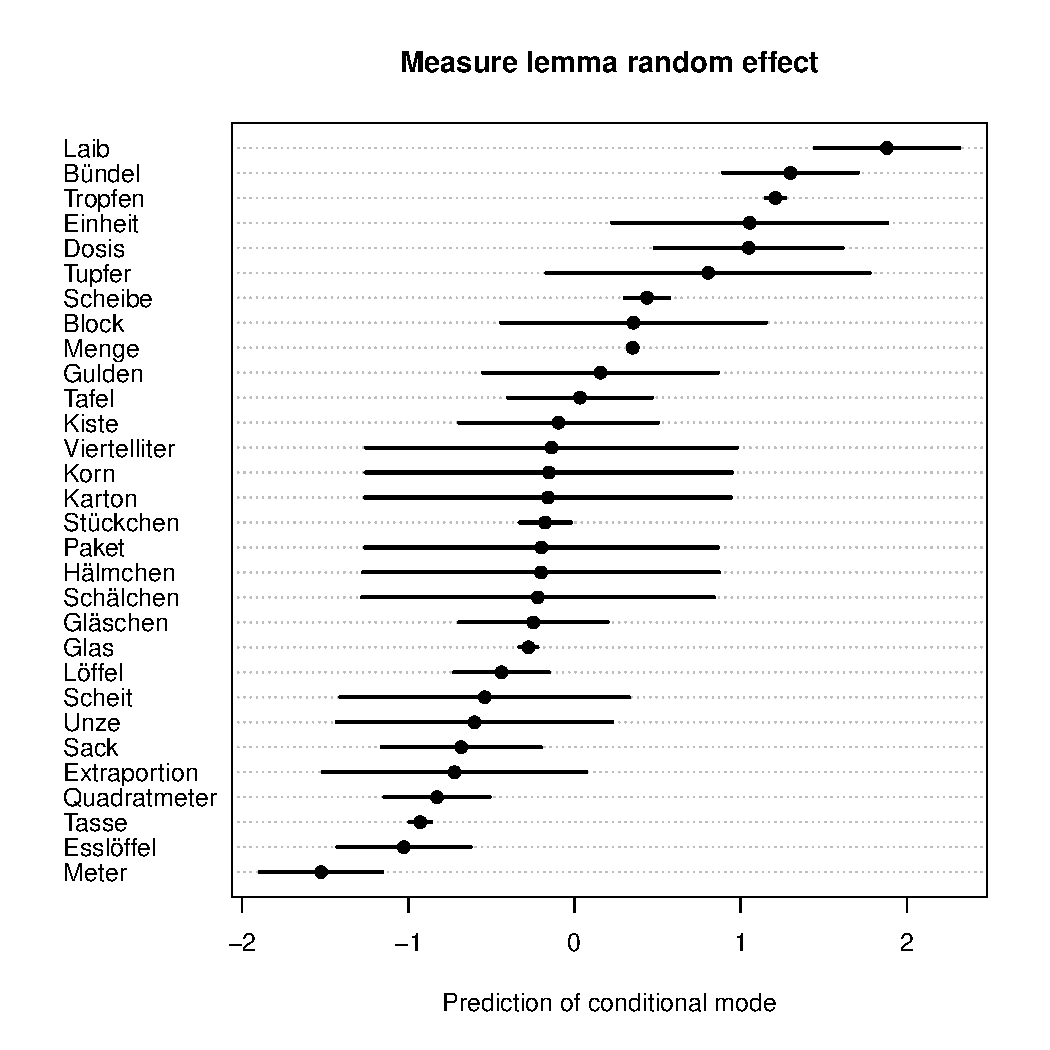
\includegraphics[width=\textwidth]{RPHCL/ranef_selection}
  \caption{Dot plot with prediction intervals for a random subset of 30 conditional modes (model \texttt{glmm.01}, random intercept for \texttt{Measurelemma})}
  \label{fig:condmodes}
\end{figure}

Turning to the quality of the overall model fit, Nakagawa \& Schielzeth's coefficients of determination can be calculated with the \texttt{r.squaredGLMM(glmm.01)} command (from the \texttt{MuMIn} package).
The output looks as follows.

\vspace{0.5\baselineskip}

\begin{lstlisting}
      R2m       R2c
0.2004865 0.4209018
\end{lstlisting}

This informs the user that the fixed effects cumulatively account for a proportion of 0.200 of the total variance in the data.
Taking also the random effect into account, the model explains a proportion of 0.421 of the total variance.
The random effect thus appears to be relevant.
Comparing the conditional $R^2$ to the Nagelkerke $R^2$ of the GLM with \texttt{Measurelemma} as a fixed effect (which was 0.397), we see that the difference is not substantial although the individual coefficient estimates in the GLM were unreliable.

Furthermore, readers are encouraged to compare the estimates of the fixed effects for \texttt{glm.01} (except \texttt{Measurelemma}) and for \texttt{glmm.01}.%
\footnote{Again, the accompanying script contains all necessary code.}
The fixed-effects coefficient estimates (except for the intercept, which is heavily offset in \texttt{glm.01}) do not differ much between the GLM and the GLMM, which indicates that the grouping variable \texttt{Measurelemma} does not enter into an interaction with the fixed effects.
However, the standard deviations (and consequently the confidence intervals as well as the p-values) change.

\paragraph{Reporting the results}

Journals and conferences in corpus linguistics apparently do not enforce strict guidelines when it comes to reporting the results of GLMM fits.
While a coefficient table for the fixed effects is a de-facto standard for GLMMs just as much as for GLMs, there is no such de-facto standard with regard to which measures of model quality for GLMMs should be reported, and especially how random effects should be reported.
Everything that should be reported for a GLM should also be reported for a GLMM, such as the coefficient table for the fixed effects (which should at least contain the coefficient estimate, the standard error, and possibly bootstrapped confidence intervals) and variance inflation factors \citep{FoxMonette1992,ZuurEa2010}.
In addition, the present author recommends to report (either in the running text, in tabular form, or in the caption of the coefficient table):

\begin{enumerate}
  \item the estimate of the random effect variance (and covariance) parameters
  \item (bootstrapped) confidence intervals for the above
  \item Nakagawa \& Schielzeth's $R^2$ coefficients of determination
  \item optionally all or some conditional modes with prediction intervals in tabular form or as a dot plot (see Figure~\ref{fig:condmodes})
  \item (bootstrapped) p-values for random effects if absolutely necessary, and only if the model comparison is possible between nested GLMMs and does not involve the direct comparison of a GLM and a GLMM (see for example the \texttt{PBmodcomp} function from the \texttt{pbkrtest} package; \citealt{HalekohHojsgaard2014}) 
\end{enumerate}

\subsubsection{More complex models}

The \texttt{glmer} call as used for the original paper is as follows.

\vspace{0.5\baselineskip}

\begin{lstlisting}
glmm.10 <- glmer(Construction~1
                 +(1|Measurelemma)   # Random.
                 +(1|Kindlemma)
                 +Badness            # Item-level.
                 +Cardinal
                 +Genitives
                 +Measurecase
                 +Kindattraction     # Kind lemma level.
                 +Kindfreq
                 +Kindgender
                 +Measureattraction  # Measure lemma level.
                 +Measureclass
                 +Measurefreq,
                 data=measure,
		 family=binomial(link=logit),
		 na.action = na.fail,
                 control=glmerControl("bobyqa"))
\end{lstlisting}

Since the model has a relatively high degree of complexity, the option \texttt{control=glmerControl("bobyqa")} is required.
It selects a different optimiser (an algorithm used by the estimator).
In general, BOBYQA optimisers are highly robust, and using a BOBYQA is the first step to try when there are convergence errors.

The second-level predictors have the same value per level of the corresponding random intercept and are automatically treated as second-level effects.
In order to illustrate the interpretation of the conditional modes and the fixed effects coefficients in such a model, there is code in the accompanying script which extracts all relevant values and calculates a predicted value for item 99 (arbitrarily chosen for illustration purposes) from the \texttt{measure} data set.
For example, the overall intercept of -3.653 can be extracted via the following command.

\vspace{0.5\baselineskip}

\begin{lstlisting}
coef(summary(glmm.03))['(Intercept)','Estimate']
\end{lstlisting}

To this intercept, the sub-terms for first-level fixed effects are added.
They can be calculated as follows, using \texttt{Badness} as an example.
The result is 0.0183.

\vspace{0.5\baselineskip}

\begin{lstlisting}
coef(summary(glmm.03))['Badness', 'Estimate'] *
  measure[99, 'Badness']
\end{lstlisting}

In other words, we extract the fixed-effect coefficient estimate for \texttt{Badness} and multiply it with the \texttt{Badness} value observed for item 99.

In order to calculate the contribution of the second-level effects, which will be added to the overall intercept and the first-level fixed-effects sub-terms, we first need to extract the appropriate group-level intercept.
The following code extracts the \texttt{Kindlemma} random intercept for item 99, which is -0.159 for the lemma \textit{Wasser} `water'.

\vspace{0.5\baselineskip}

\begin{lstlisting}
ranef(glmm.03)$Kindlemma[
  as.character(measure[99, 'Kindlemma']), '(Intercept)']
\end{lstlisting}

To these group-level intercepts, the second-level fixed-effects sub-terms are added, and they can be calculated very much like their first-level equivalents.
For example, the following code calculates the sub-term for \texttt{Kindfreq}, which is -0.044 (the z-transformed logarithmised frequency per one million tokens of \textit{Wasser}) in this case.

\vspace{0.5\baselineskip}

\begin{lstlisting}
coef(summary(glmm.03))['Kindfreq', 'Estimate'] *
  measure[99, 'Kindfreq']
\end{lstlisting}

All in all, the prediction for the \texttt{Measurelemma} second-level model is -0.027.
For the \texttt{Kindlemma} second-level model, it is 0.125, and for the first-level fixed-effects part of the model (including the overall intercept), it is -3.382.
Added up, the linear term is predicted to be -3.284.
This result needs to go through the inverse logit link function (implemented as \texttt{invlogit} in the \texttt{car} package, for example), which results in 0.036.
Given the coding of the response variable, this means that the model predicts a probability of 0.036 that the genitive construction is chosen in the given example.
Readers are advised to go through the full calculations in order to understand what the different numbers in their reported GLMMs represent.
They will likely realise that the superficial maths involved is relatively transparent, even for more complex models.
